\documentclass[9pt, letterpaper, landscape]{article}
\usepackage[margin=0.4in, top=0.3in, bottom=0.25in]{geometry}
\usepackage{graphicx, booktabs, enumitem, multicol}
\usepackage[dvipsnames]{xcolor}
\usepackage[most]{tcolorbox}
\pagestyle{empty}

% ── Color scheme ──
\definecolor{Navy}{HTML}{1B2A4A}
\definecolor{Teal}{HTML}{2E8B8B}
\definecolor{Gold}{HTML}{D4A843}
\definecolor{PosGreen}{HTML}{2E7D32}
\definecolor{NegRed}{HTML}{C62828}
\definecolor{LightGray}{HTML}{F5F5F5}

\setlength{\parindent}{0pt}
\setlength{\parskip}{0pt}
\setlength{\columnsep}{12pt}
\renewcommand{\arraystretch}{1.1}

% ── Section header command ──
\newcommand{\hsec}[1]{%
  \vspace{4pt}%
  {\footnotesize\bfseries\color{Navy}\MakeUppercase{#1}}%
  \par\vspace{1pt}%
  {\color{Teal}\hrule height 0.4pt}%
  \vspace{2pt}%
}
\newcommand{\hsecnote}[2]{%
  \vspace{4pt}%
  {\footnotesize\bfseries\color{Navy}\MakeUppercase{#1}\quad{\normalfont\scriptsize\color{gray}#2}}%
  \par\vspace{1pt}%
  {\color{Teal}\hrule height 0.4pt}%
  \vspace{2pt}%
}

\begin{document}

% ══════════════════════════════════════════════════════════════
% TOP BANNER
% ══════════════════════════════════════════════════════════════
\begin{tcolorbox}[
  colback=Navy, colframe=Navy, sharp corners, boxrule=0pt,
  top=4pt, bottom=3pt, left=10pt, right=10pt,
  before skip=0pt, after skip=4pt
]
\centering
{\normalsize\bfseries\color{white} Regime-Dependent Delta Hedging with SVI-Calibrated Volatility Surfaces on SPX Index Options}\\[2pt]
{\small\color{Gold} Zaid Annigeri \quad{\color{white}|}\quad Master of Quantitative Finance, Rutgers Business School \quad{\color{white}|}\quad\color{white} ma.zaid@rutgers.edu}
\end{tcolorbox}

% ══════════════════════════════════════════════════════════════
% THREE-COLUMN BODY
% ══════════════════════════════════════════════════════════════
\begin{multicols}{3}

% ──────────────────────────────────────────────────────────────
% COLUMN 1
% ──────────────────────────────────────────────────────────────

\hsec{The Gap}

{\scriptsize
SVI is the industry standard for volatility surface calibration. The literature validates fitting quality (10--50 bps RMSE) but stops there. \textbf{No study has tested whether a better surface fit produces a better hedge.} We close that loop on 2,000 real SPX options across four VIX regimes.}

\hsec{The Experiment}

{\scriptsize
\textbf{28.6M} SPX options $\to$ \textbf{5.6M} filtered $\to$ \textbf{2,000} stratified (500 per regime)

\vspace{2pt}
\begin{tabular}{@{}r@{\;$\to$\;}l@{}}
5 vol inputs & BSM $\Delta$ (daily hedge to expiry)\\
4 VIX regimes & Low / Normal / High / Crisis\\
Decomposition & El Karoui et al.\ (1998)\\
\end{tabular}
}

\hsec{Three Hypotheses}

{\scriptsize
\textbf{H1:} SVI reduces error vs.\ flat BSM \hfill \textcolor{NegRed}{\textbf{REJECTED}}

\textbf{H2:} Yang-Zhang beats Close-to-Close \hfill \textcolor{NegRed}{\textbf{REJECTED}}

\textbf{H3:} Optimal input is regime-dependent \hfill \textcolor{PosGreen}{\textbf{PARTIAL}}
}

\hsec{Why Does the Smile Hurt?}

{\scriptsize
\begin{enumerate}[nosep, leftmargin=12pt, itemsep=1pt]
\item \textbf{Calibration noise:} 5-param optimization $\to$ noisy $\Delta$
\item \textbf{Interpolation:} calibrate every 5th day $\to$ stale smile
\item \textbf{Signal $<$ noise} for most strikes---only OTM calls have steep enough slope to carry information
\end{enumerate}

\vspace{2pt}
\colorbox{LightGray}{\parbox{0.95\linewidth}{\scriptsize\textit{Parkinson is 5$\times$ more efficient than CC under GBM (Parkinson 1980), yet produces the worst hedging ($-$43.2\%). Statistical efficiency $\neq$ hedging efficiency.}}}}

% ──────────────────────────────────────────────────────────────
% COLUMN 2
% ──────────────────────────────────────────────────────────────

\hsecnote{The Horse Race}{Gain vs.\ Flat BSM Benchmark}

\vspace{1pt}
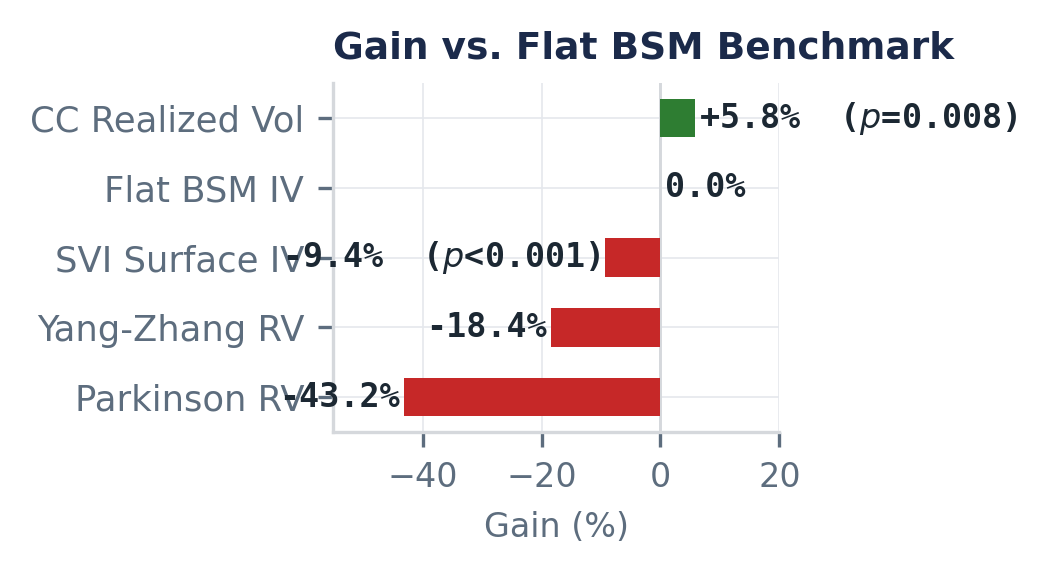
\includegraphics[width=\columnwidth]{figures/horse_race.png}

\vspace{2pt}
{\tiny\textit{Hull \& White (2017) report 25.7\% Gain on SPX calls using minimum-variance delta---up to 42.1\% for deep OTM. Our CC RV achieves +5.8\% with a simpler method; the moneyness-conditional strategy targets the same OTM region where their gains are largest.}}

\hsecnote{Regime Breakdown}{Why H3 is ``partial''}

\vspace{1pt}
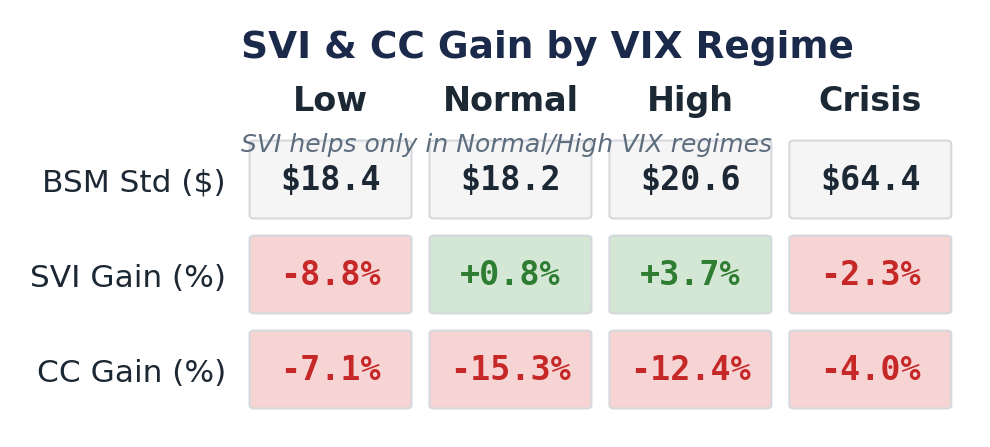
\includegraphics[width=\columnwidth]{figures/regime_breakdown.png}

\hsecnote{The Twist}{Best Vol Input by Moneyness $\times$ DTE}

\vspace{1pt}
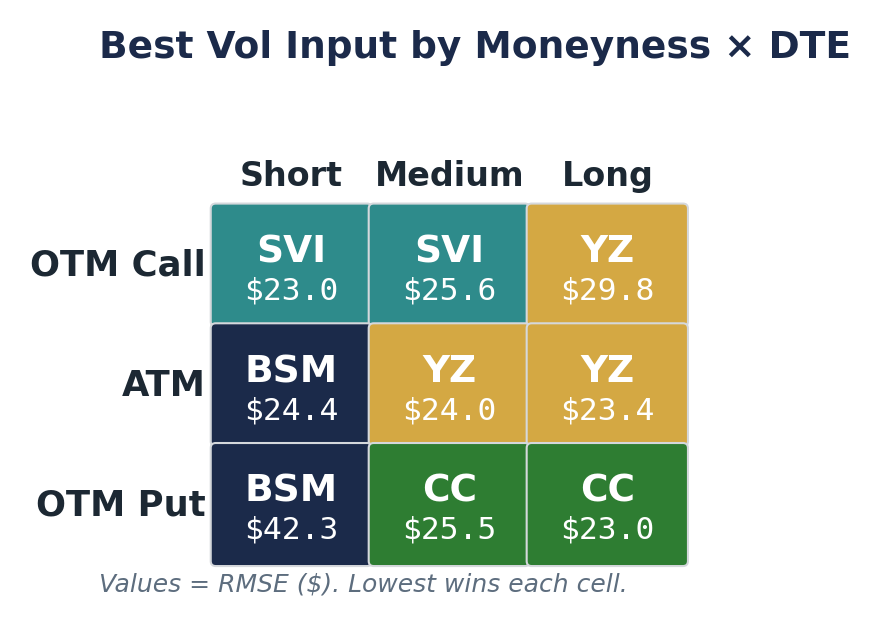
\includegraphics[width=\columnwidth]{figures/moneyness_dte.png}

% ──────────────────────────────────────────────────────────────
% COLUMN 3
% ──────────────────────────────────────────────────────────────

\hsecnote{P\&L Attribution}{Variance Contribution by Regime}

\vspace{1pt}
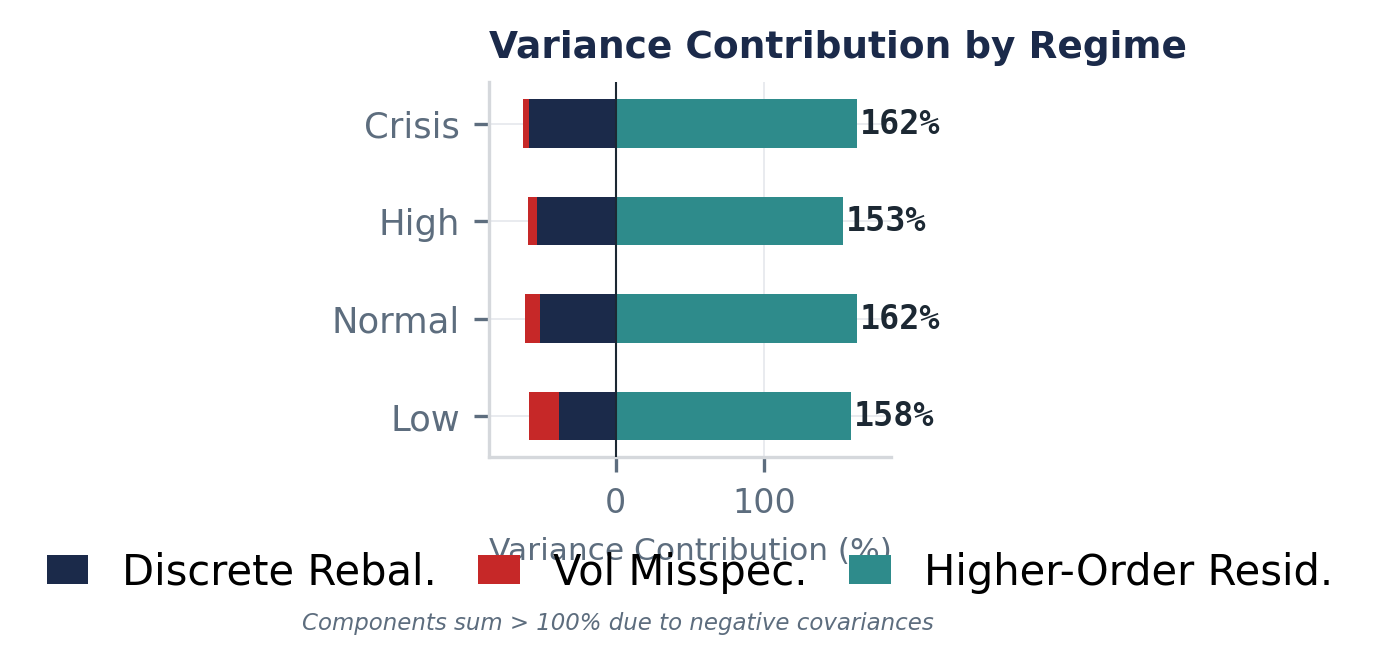
\includegraphics[width=\columnwidth]{figures/pnl_attribution.png}

\hsec{Key Numbers}

{\scriptsize
\begin{tabular}{@{}lr@{}}
\toprule
\textbf{Metric} & \textbf{Value} \\
\midrule
Sample & 2,000 SPX options \\
Period & Jan 2019 -- Dec 2024 \\
SVI RMSE & 19.5 bps median \\
Arb-free rate & 68.6\% \\
Best overall & CC RV (+5.8\%) \\
Worst overall & Park ($-$43.2\%) \\
$\Delta$-$\Gamma$ hedge & 46\% std reduction \\
Unit tests & 80 (all passing) \\
\bottomrule
\end{tabular}
}

\hsec{Practitioner Takeaway}

{\scriptsize
\begin{tabular}{@{}l@{\;\;$\to$\;\;}l@{}}
OTM Calls & SVI Surface IV (+6--12\%) \\
ATM & Flat BSM IV \\
OTM Puts & CC Realized Vol (+21--48\%) \\
VIX $\geq$ 35 & Focus on gamma management \\
\end{tabular}

\vspace{3pt}
\colorbox{LightGray}{\parbox{0.95\linewidth}{\scriptsize\textbf{Bottom line:} No single vol input wins everywhere. A moneyness-conditional strategy outperforms any single approach.}}

\vspace{2pt}
\colorbox{LightGray}{\parbox{0.95\linewidth}{\tiny\textbf{Economic impact:} For a \$1B notional SPX book, 5.8\% hedging error reduction $\approx$ 5--8\% lower VaR, freeing risk capital.}}

\vspace{2pt}
{\tiny\textit{Ruf \& Wang (2022) show simple regressions match neural networks on real SPX---our regime-conditional approach targets the same channel with full interpretability.}}
}

\end{multicols}

\vfill
\begin{center}
{\small\color{Teal}\textit{The counterintuitive finding: the industry-standard volatility surface makes hedging worse. Ask me why.}}
\end{center}
\vspace{2pt}

% ══════════════════════════════════════════════════════════════
% BOTTOM BANNER
% ══════════════════════════════════════════════════════════════
\begin{tcolorbox}[
  colback=Navy, colframe=Navy, sharp corners, boxrule=0pt,
  top=3pt, bottom=3pt, left=10pt, right=10pt,
  before skip=2pt, after skip=0pt
]
\begin{minipage}[c]{0.32\textwidth}
{\scriptsize\color{white}
ma.zaid@rutgers.edu\\
linkedin.com/in/zaidannigeri\\
github.com/zaid282802/options-pricing-hedging}
\end{minipage}\hfill
\begin{minipage}[c]{0.36\textwidth}
\centering
{\scriptsize\color{white} Future Alpha 2026 \quad|\quad Brooklyn Marriott \quad|\quad March 31--April 1}\\[1pt]
{\tiny\color{Gold}\textit{Full 40-page thesis and Python code available upon request}}
\end{minipage}\hfill
\begin{minipage}[c]{1.6cm}
\raggedleft

\includegraphics[width=1.5cm]{qr_github.png}
\end{minipage}
\end{tcolorbox}

\end{document}
